\section{Datengrundlage und Datenakquise}
\label{chap:daten}

\subsection{Die Datenquelle: Pokémon-API (pokeAPI.co)}
\label{sec:datenquelle}
Die Wahl fiel auf die PokeAPI als primäre Datenquelle für dieses Projekt, da sie eine vollumfassende und gut strukturierte Sammlung von Pokémon-Daten bereitstellt. Diese RESTful API zeichnet sich durch ihre vollständige Dokumentation und den freien Zugang ohne Authentifizierung aus, was sie ideal für dieses Projekt macht.


\subsection{Analyse der Datenstruktur und relevanter Endpunkte}
\label{sec:datenstruktur}

Die API bietet verschiedene Endpunkte, wobei für dieses Projekt hauptsächlich die Endpunkte \texttt{/pokemon/\{id\}} und \texttt{/pokemon-species/\{id\}} genutzt wurden. Das JSON-Format der Antworten folgt einem konsistenten Schema mit verschachtelten Objekten für komplexe Datenstrukturen wie Statistiken, Typen und Fähigkeiten.

Die Transformation der rohen API-Daten in ein suchoptimiertes Solr-Dokument erfordert umfangreiche Umstrukturierung und Anreicherung. Listing~\ref{lst:solr_document} zeigt das finale indexierte Dokument für Bulbasaur nach der Verarbeitung. Besonders erkennbar ist die Flattening-Strategie: Während die ursprünglichen API-Daten verschachtelte Arrays und Objekte für Typen und Statistiken verwenden, werden diese in direkt durchsuchbare Felder wie \texttt{primary\_type}, \texttt{secondary\_type} und individuelle \texttt{stat\_\{name\}}-Felder aufgeteilt.
Die Datenergänzung wird durch berechnete Felder wie \texttt{total\_stats} (Summe aller Basiswerte) und \texttt{generation} (abgeleitet aus der Pokémon-ID) deutlich. Besonders ist die Multi-Value-Behandlung: Das \texttt{levelup\_moves}-Array enthält alle durch Levelaufstieg erlernbaren Attacken in alphabetischer Sortierung, während \texttt{all\_abilities} sowohl normale als auch versteckte Fähigkeiten kombiniert. Das \texttt{flavor\_text}-Array aggregiert alle englischsprachigen Beschreibungen aus verschiedenen Spielversionen und bietet damit eine umfassende Textbasis für die Volltextsuche.

\noindent
\begin{minipage}{\linewidth}
\begin{lstlisting}[language=json, caption=Beispiel eines indexierten Pokemon-Dokuments in Solr, label=lst:solr_document, basicstyle=\footnotesize\ttfamily, breaklines=true]
{
  "id": "1",
  "pokemon_id": 1,
  "name": "Bulbasaur",
  "name_spell": ["Bulbasaur"],
  "height": 7,
  "weight": 69,
  "base_experience": 64,
  "types": ["grass", "poison"],
  "primary_type": "grass",
  "secondary_type": "poison",
  "abilities": ["Overgrow"],
  "hidden_abilities": ["Chlorophyll"],
  "all_abilities": ["Overgrow", "Chlorophyll"],
  "stat_hp": 45,
  "stat_attack": 49,
  "stat_defense": 49,
  "stat_special_attack": 65,
  "stat_special_defense": 65,
  "stat_speed": 45,
  "total_stats": 318,
  "levelup_moves": [
    "Double Edge", "Growl", "Growth", "Leech Seed", 
    "Poison Powder", "Power Whip", "Razor Leaf", 
    "Seed Bomb", "Sleep Powder", "Solar Beam", 
    "Sweet Scent", "Synthesis", "Tackle", "Take Down", 
    "Vine Whip", "Worry Seed"
  ],
  "color": "green",
  "habitat": "grassland",
  "base_happiness": [70],
  "capture_rate": 45,
  "is_legendary": false,
  "is_mythical": false,
  "generation": 1,
  "flavor_text": [
    "A strange seed..."
  ],
  "spellcheck_base": [
    "Bulbasaur",
    "A strange seed was planted on its back at birth..."
  ],
  "_version_": 1838720269085048832
}
\end{lstlisting}
\label{fig:language-distribution}

\end{minipage}

\subsection{Datenakquise und Vorverarbeitung mit \texttt{api\textunderscore client.py}}
\label{sec:datenakquise}

Die ApiClient-Klasse nutzt eine persistente requests.Session für effiziente HTTP-Verbindungswiederverwendung und implementiert 
mehrere kritische Sicherheitsmechanismen für den produktiven Einsatz.
Der zentrale \texttt{fetch\_with\_retry()}-Mechanismus führt bis zu drei Wiederholungsversuche bei fehlgeschlagenen Anfragen durch. Die implementierte exponentielle Backoff-Strategie wartet $2^{\text{attempt}}$ Sekunden zwischen den Versuchen, was bei temporären Netzwerkproblemen oder Server-Überlastungen besonders wirkungsvoll ist. Zusätzlich kommt ein 10-Sekunden-Timeout für alle HTTP-Requests zum Einsatz, um hängende Verbindungen zu vermeiden.
Um die Nutzungsrichtlinien der PokeAPI zu respektieren und Server-Überlastung zu vermeiden, wird jede API-Anfrage durch den konfigurierbaren \texttt{REQUEST\_DELAY} von 100 Millisekunden verzögert. Die Implementierung zweier spezialisierter Endpunkt-Methoden optimiert die Datenerfassung: \texttt{fetch\_pokemon\_basic\_data()} ruft Statistiken, Typen und Fähigkeiten über den Endpunkt \texttt{/pokemon/\{id\}} ab, während \texttt{fetch\_pokemon\_species\_data()} Beschreibungen, Farben und Habitat-Informationen über \texttt{/pokemon-species/\{id\}} bezieht.

\textbf{Retry-Mechanismus:} Die Methode \texttt{fetch\textunderscore with\textunderscore retry()} führt bis zu 3 Wiederholungsversuche bei fehlgeschlagenen Anfragen durch, mit exponentieller Backoff-Strategie (2\textasciicircum attempt Sekunden Wartezeit).

\textbf{Rate-Limiting:} Jede API-Anfrage wird durch \texttt{REQUEST\textunderscore DELAY} verzögert, um die API-Richtlinien zu respektieren und Server-Überlastung zu vermeiden.

\textbf{Spezialisierte Endpunkte:} Zwei Hauptmethoden greifen auf verschiedene API-Endpunkte zu:
\begin{itemize}
    \item \texttt{fetch\textunderscore pokemon\textunderscore basic\textunderscore data()}: Abruf von \texttt{/pokemon/\{id\}} für Grunddaten (Stats, Typen, Fähigkeiten)
    \item \texttt{fetch\textunderscore pokemon\textunderscore species\textunderscore data()}: Abruf von \texttt{/pokemon-species/\{id\}} für Artendaten (Beschreibungen, Farbe, Habitat)
\end{itemize}

\subsection{Datenbereinigung und Transformation mit \texttt{data\_processor.py}}

Die rohen JSON-Daten der PokeAPI müssen für die Verwendung in Solr aufbereitet werden. Die \texttt{DataProcessor}-Klasse implementiert eine mehrstufige Verarbeitungspipeline, die sowohl Datenqualität als auch Suchperformance optimiert.

Die Textbereinigung erfolgt über die \texttt{clean\_text()} Methode, die mittels regulärer Ausdrücke Steuerzeichen wie Zeilenumbrüche, Seitenvorschübe und Tabulatoren entfernt. Mehrfache Leerzeichen werden normalisiert und führende sowie nachgestellte Leerzeichen entfernt. Diese Bereinigung ist wichtig für die Flavor-Texte, die oft Formatierungsartefakte aus der ursprünglichen Spieldarstellung enthalten.

Das Flattening verschachtelter JSON-Strukturen stellt einen wichtigen Verarbeitungsschritt dar. Pokemon-Typen werden aus dem ursprünglich verschachtelten Array-Format in die separaten Felder \texttt{primary\_type}, \texttt{secondary\_type} und das durchsuchbare \texttt{types}-Array aufgeteilt. Statistiken erhalten eine doppelte Behandlung: Einzelne Werte werden in spezifische Felder wie \texttt{stat\_hp} und \texttt{stat\_attack} extrahiert, während gleichzeitig ein \texttt{total\_stats}-Wert für Vergleiche berechnet wird.

Die Behandlung von Fähigkeiten erfolgt durch Kategorisierung in normale und versteckte Fähigkeiten. Dabei werden Bindestriche durch Leerzeichen ersetzt und die Namen mit \texttt{title()} formatiert. Das kombinierte \texttt{all\_abilities}-Feld ermöglicht eine umfassende Fähigkeiten-Suche unabhängig vom Typ.

Die Generationszuordnung erfolgt über ID-basierte Bereiche (Generation 1: 1--151, Generation 2: 152--251, Generation 3: 252--386), was eine effiziente Kategorisierung ohne zusätzliche API-Aufrufe ermöglicht. Für Move-Sets werden nur durch Level-Up erlernbare Moves extrahiert und in einem Set dedupliziert, bevor sie als sortierte Liste gespeichert werden.

\subsection{Technische Besonderheiten: Rate-Limiting und Fehlerbehandlung}

Das System implementiert mehrere Maßnahmen für einen stabilen Betrieb. Neben dem bereits erwähnten Rate-Limiting kommt ein 10-Sekunden-Timeout für HTTP-Requests zum Einsatz. Umfassendes Logging unterstützt Debugging und Monitoring, während eine Graceful Degradation-Strategie die Fortsetzung der Indexierung auch bei einzelnen Fehlern ermöglicht.

\section{Systemarchitektur und Konzeption}

\subsection{Überblick der containerisierten Gesamtarchitektur}

Die Entscheidung für eine containerisierte Architektur mit Docker Compose bringt Vorteile in Bezug auf Portabilität und Reproduzierbarkeit mit sich.
Der Solr-Container läuft mit Apache Solr 9.4 auf Port 8983, wobei 512MB Heap-Speicher und persistente Volumes für Datenerhaltung sorgen. Das Pokemon-spezifische Schema wird automatisch durch die \texttt{SolrIndexer}-Klasse erstellt und konfiguriert.

Die Flask-Anwendung operiert in einem separaten Web-Container auf Port 5000 und kommuniziert über das interne Docker-Netzwerk mit Solr. Die automatische Abhängigkeitsverwaltung durch \texttt{depends\_on} mit Health-Check gewährleistet eine korrekte Startsequenz der Services.

Die Netzwerk-Isolation durch ein dediziertes Bridge-Netzwerk namens \texttt{pokemon-network} verbessert sowohl Sicherheit als auch Performance. Diese Architektur ermöglicht es, beide Services isoliert zu betreiben, während sie effizient miteinander kommunizieren können.

Das Installationsskript \texttt{install.sh} automatisiert den kompletten Setup-Prozess und macht das System auch für weniger technisch versierte Nutzer zugänglich. Es überprüft Systemvoraussetzungen wie Python 3 und Docker oder Podman, erstellt eine Python Virtual Environment, installiert Abhängigkeiten aus der \texttt{requirements.txt}, startet die Container-Services, wartet auf Solr-Bereitschaft mit Health-Check und führt schließlich den Datenimport-Prozess aus. Die Unterstützung verschiedener Betriebssysteme und Container-Runtimes sowie umfassende Fehlerbehandlung mit farbiger Konsolen-Ausgabe runden die Benutzerfreundlichkeit ab.

\subsection{Entwurf des Solr-Indexschemas}

Das Solr-Schema wurde entwickelt, um verschiedene Suchszenarien optimal zu unterstützen. Die Feldtyp-Definition umfasst \texttt{pint} für numerische Werte mit automatischer Sortierung und Facettierung, \texttt{string} für exakte Matches ohne Textanalyse, \texttt{text\_general} für Volltextsuche mit Tokenisierung, \texttt{boolean} für binäre Eigenschaften und \texttt{strings} für Multi-Value-Arrays.

Die Indexstruktur spiegelt die komplexe Natur der Pokemon-Daten wider und wurde für optimale Performance konfiguriert. Zentrale Identifikationsfelder wie \texttt{pokemon\_id} nutzen \texttt{docValues} ohne Indexierung (\texttt{indexed: false}) für effiziente Sortierung bei minimaler Index-Größe. Das \texttt{name}-Feld hingegen bleibt vollständig indexiert für Suchfunktionalität. Physische Eigenschaften wie \texttt{height}, \texttt{weight} und alle statistischen Einzelwerte (\texttt{stat\_hp}, \texttt{stat\_attack}, \texttt{stat\_defense}, \texttt{stat\_special\_attack}, \texttt{stat\_special\_defense}, \texttt{stat\_speed}) werden als nicht-indexierte numerische Felder mit \texttt{docValues} implementiert, da sie primär für Sortierung und Anzeige benötigt werden.

Suchrelevante Felder wie Typ-Felder (\texttt{primary\_type}, \texttt{secondary\_type}, \texttt{types}), 

Fähigkeiten (\texttt{abilities}, \texttt{hidden\_abilities}, \texttt{all\_abilities}) und Boolean-Felder (\texttt{is\_legendary}, \texttt{is\_mythical}) bleiben vollständig indexiert für facettierte und exakte Suche. Reine Anzeige-Felder wie \texttt{color} und \texttt{habitat} nutzen \texttt{docValues} ohne Indexierung für speichereffiziente Facettierung.

Die Implementierung von Copy-Fields ermöglicht übergreifende Suche. Das \texttt{name}-Feld wird automatisch in \texttt{name\_spell} kopiert, was Rechtschreibkorrektur ermöglicht, ohne die ursprüngliche Suchperformance zu beeinträchtigen. Das \texttt{spellcheck\_base}-Feld aggregiert verschiedene durchsuchbare Inhalte für die Spell-Check-Dictionary-Erstellung. Diese selektive Indexierung reduziert die Index-Größe bei gleichzeitiger Beibehaltung aller erforderlichen Query-Funktionalitäten durch \texttt{docValues}.

\section{Implementierung der Kernkomponenten}

\subsection{Indexierungspipeline mit \texttt{solr\_indexer.py}}

Die \texttt{SolrIndexer}-Klasse orchestriert die komplette Solr-Integration. Das automatische Schema-Setup über \texttt{setup\_solr\_schema()} prüft zunächst die Existenz jedes Feldes über REST-API-Aufrufe an den \texttt{/schema/fields/\{field\_name\}} Endpunkt, bevor neue Felder hinzugefügt werden. Da bei jeder Ausführung stets derselbe Endzustand erreicht wird, sind Wiederholungen konfliktfrei möglich.

Die Feldkonfiguration erfolgt systematisch: Numerische Felder erhalten \texttt{docValues=True} für effiziente Sortierung und Facettierung, Text-Felder werden für Volltextsuche mit \texttt{text\_general} konfiguriert, und Multi-Value-Felder unterstützen Arrays für komplexe Datenstrukturen. Die Copy-Field-Konfiguration von \texttt{name} zu \texttt{name\_spell} wird ebenfalls automatisch angelegt und auf Existenz geprüft.

Der Indexierungsprozess implementiert Batch-Verarbeitung mit 50-Dokument-Batches, um Speicher-Effizienz zu gewährleisten und große Datasets handhaben zu können. Die \texttt{tqdm}-Integration bietet visuelles Feedback über den Fortschritt der Indexierung. Nach der vollständigen Indexierung wird der Index über \texttt{solr.optimize()} für bessere Suchperformance optimiert.

Die Spellcheck-Integration stellt ein wichtiges Feature dar. Die \texttt{build\_spellcheck\_dictionary()} Methode lädt zunächst den Solr-Core über die Admin-API neu, um Schema-Änderungen zu aktivieren, und triggert dann die Dictionary-Erstellung über den SpellCheck-Component mit dem Parameter \texttt{spellcheck.build=true}. Dies ermöglicht kontextuelle Rechtschreibkorrektur basierend auf den tatsächlich indexierten Daten.

\subsection{Entwicklung der Webanwendung mit Flask}

Die Flask-Anwendung wurde als vollständige RESTful API konzipiert, die sowohl programmatischen Zugriff als auch eine benutzerfreundliche Weboberfläche bietet. Die klassen-basierte Struktur der \texttt{PokemonSearchApp}-Klasse in \texttt{web\_app.py} kapselt die gesamte Anwendungslogik und Solr-Integration in einer wartbaren Form.

Das API-Design umfasst mehrere spezialisierte Endpunkte: Der Hauptsuchendpunkt \texttt{/api/search} akzeptiert Parameter für Query, Paginierung, Sortierung und Filter, während \texttt{/api/pokemon/<id>} Detailansichten für einzelne Pokemon bereitstellt. Der \texttt{/api/stats} Endpunkt liefert interessante Statistiken über die Pokemon-Sammlung, und \texttt{/api/autocomplete} bietet Echtzeit-Suchvorschläge.

Die Frontend-Integration erfolgt über ein HTML-Template in \texttt{templates/index.html}, das JavaScript für dynamische Interaktion mit den API-Endpunkten nutzt. Diese Architektur ermöglicht sowohl die Verwendung als API-Service als auch als interaktive Webanwendung.

\begin{figure}[htbp]
    \centering
    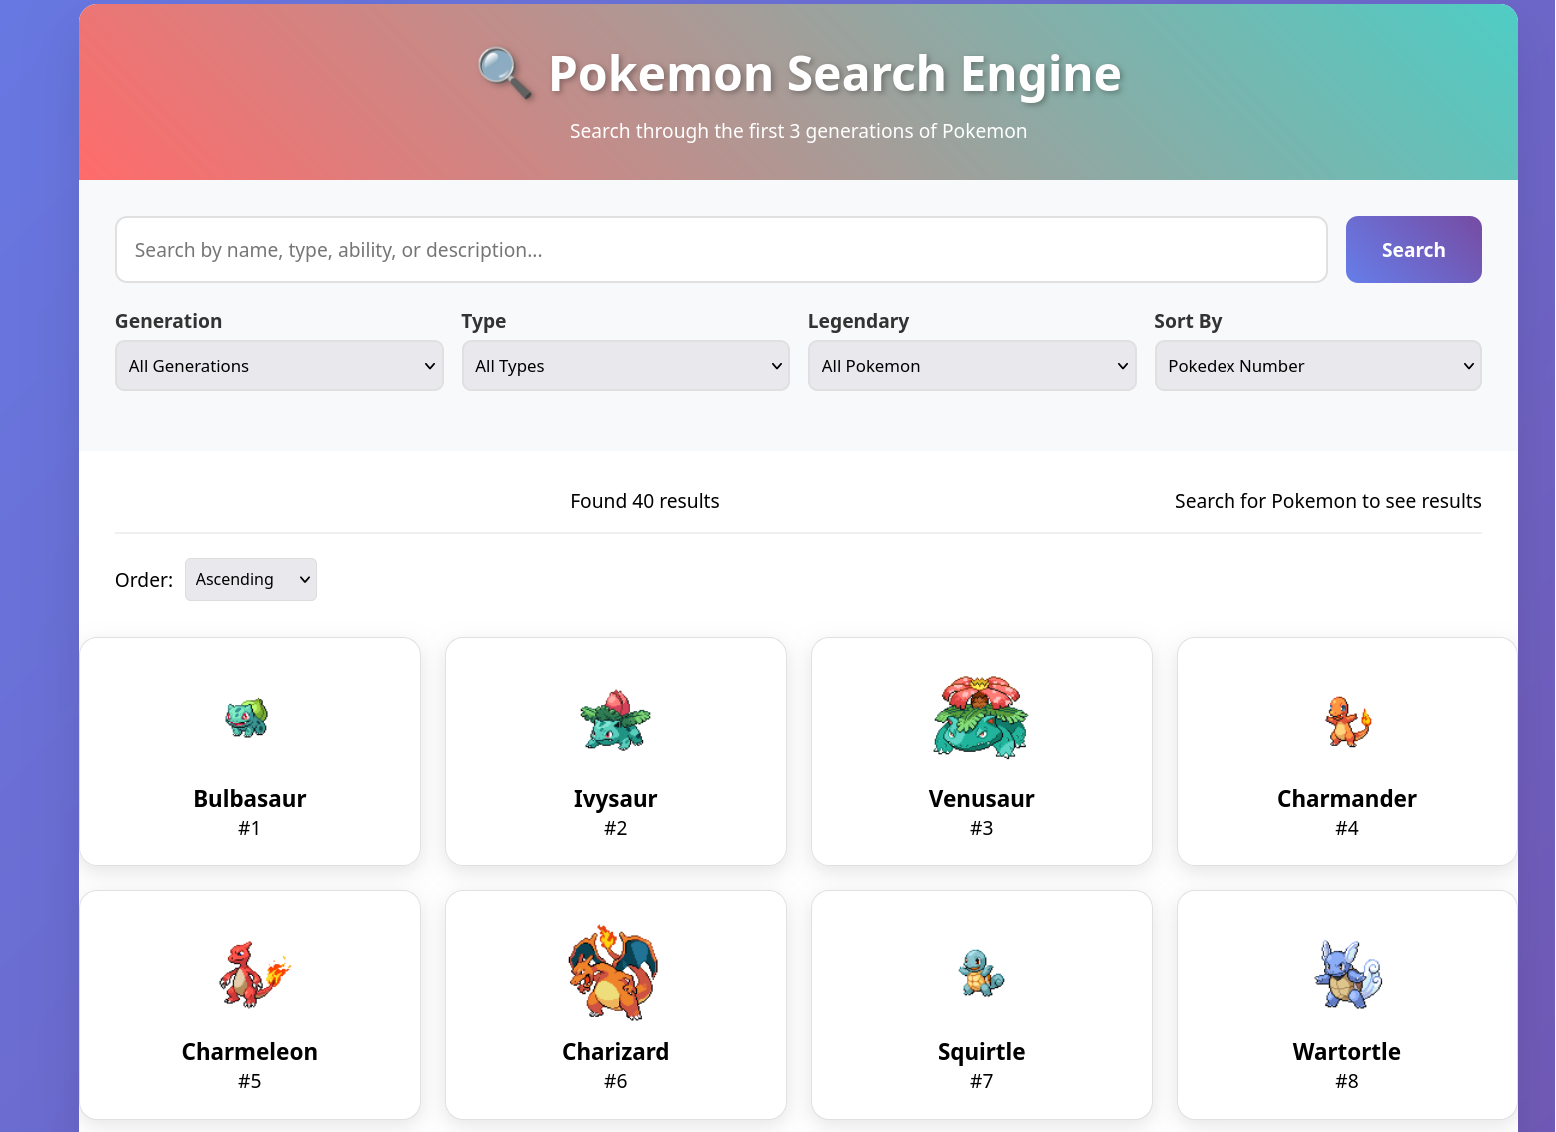
\includegraphics[width=0.95\textwidth]{figures/Screenshot_whole_page.png}
    \caption{Vollständige Benutzeroberfläche der Pokemon-Suchmaschine mit allen Hauptkomponenten: Suchfeld, Filter-Optionen (Generation, Typ, Legendary-Status), Sortierungsoptionen und Pokemon-Ergebniskarten mit Bildern und Basisdaten}
    \label{fig:whole_page}
\end{figure}

Abbildung~\ref{fig:whole_page} zeigt die vollständige Benutzeroberfläche der entwickelten Webanwendung. Die Oberfläche folgt einem klaren, dreistufigen Layout: Das zentrale Suchfeld ermöglicht freie Texteingaben, die Filterleiste bietet facettierte Suchoptionen nach Generation, Typ und Legendary-Status, und die Ergebnisdarstellung präsentiert Pokemon-Karten mit Bild, Name, Pokedex-Nummer und grundlegenden Informationen in einem responsiven Grid-Layout.

\subsection{Implementierung der Suchfunktionalitäten}

Das Suchsystem nutzt verschiedene Solr-Features für unterschiedliche Anwendungsszenarien und bietet sowohl einfache als auch fortgeschrittene Suchmöglichkeiten. Die Standard-Keyword-Suche verwendet den \texttt{edismax} Query-Parser mit einer durchdachten Feldgewichtung über den \texttt{qf} Parameter: \texttt{name\textasciicircum 5 types\textasciicircum 2 all\_abilities\textasciicircum 2 flavor\_text\textasciicircum 1}. Diese Priorisierung sorgt dafür, dass Namensübereinstimmungen die höchste Relevanz erhalten, während Typen und Fähigkeiten mittlere Priorität haben und Flavor-Text-Matches am niedrigsten gewichtet werden.

Für erweiterte Substring-Matching wird eine intelligente Wildcard-Suche mit dem Pattern \texttt{name:*query*} implementiert, die Teilübereinstimmungen an beliebiger Position im Namen findet. Dies ermöglicht es, dass eine Suche nach "`saur"' alle Pokemon mit "`-saur"'-Endung findet (Bulbasaur, Ivysaur, Venusaur).

\begin{figure}[htbp]
    \centering
    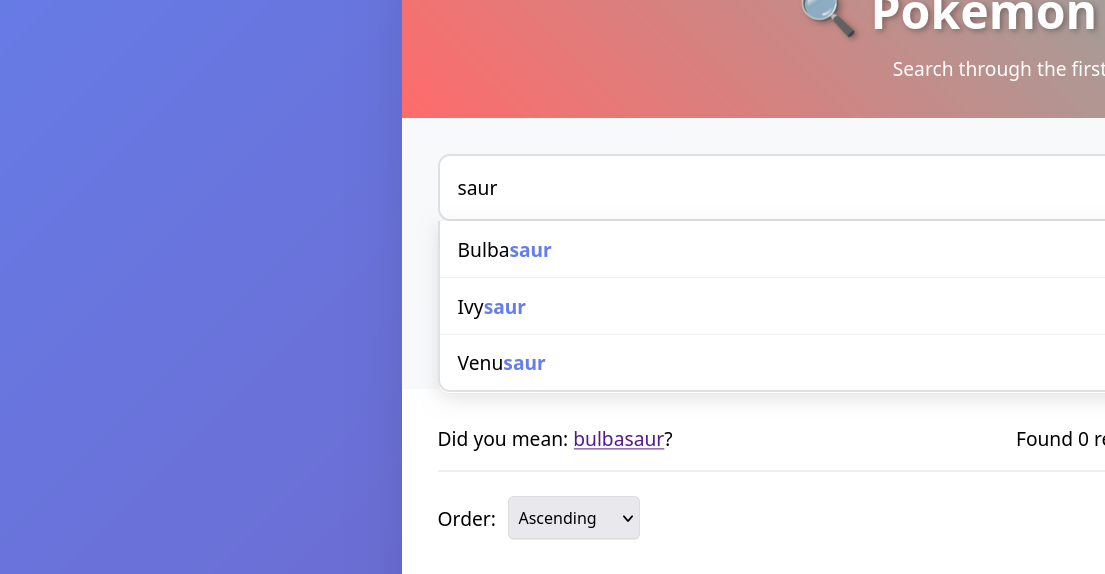
\includegraphics[width=0.6\textwidth]{figures/Screenshot_multiple_suggestions.png}
    \caption{Erweiterte Autocomplete-Funktionalität bei der Eingabe von "`saur"' mit mehreren relevanten Vorschlägen: Bulbasaur, Ivysaur und Venusaur demonstrieren das Substring-Matching}
    \label{fig:multiple_suggestions}
\end{figure}

Die Autocomplete-Funktionalität kombiniert mehrere Ansätze: Solrs Terms Component für häufige Begriffe und Wildcard-Suche für Substring-Matching. Die Implementierung unterstützt Case-Insensitive-Suche und bietet Echtzeit-Vorschläge während der Eingabe. Wie in Abbildung~\ref{fig:multiple_suggestions} dargestellt, werden bei der Eingabe von "`saur"' automatisch alle Pokemon mit dieser Endung vorgeschlagen, was die Effizienz der Suche erheblich steigert.

\begin{figure}[htbp]
    \centering
    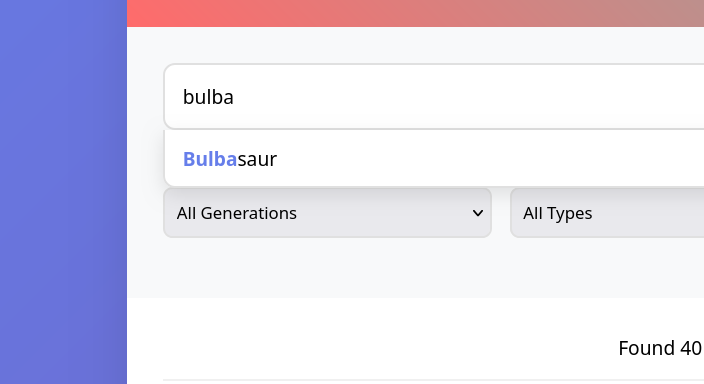
\includegraphics[width=0.5\textwidth]{figures/screenshot_search_suggestion.png}
    \caption{Einfache Autocomplete-Suggestion bei der Eingabe von "`bulba"' mit direktem Vorschlag für Bulbasaur}
    \label{fig:simple_autocomplete}
\end{figure}

Abbildung~\ref{fig:simple_autocomplete} zeigt die grundlegende Autocomplete-Funktionalität bei der Eingabe von "`bulba"'. Das System erkennt die Eingabe und schlägt unmittelbar "`Bulbasaur"' vor, wodurch Nutzer schnell zu ihrem gesuchten Pokemon navigieren können.

Die facettierte Suche wurde für die Dimensionen \texttt{generation}, \texttt{primary\_type}, \texttt{color} und \texttt{habitat} implementiert und nutzt Solrs native Facettierungs-Features mit automatischer Zählung verfügbarer Optionen. Filter können über Solrs \texttt{fq} (Filter Query) Parameter kombiniert werden, wodurch komplexe Anfragen wie "`Generation 1 UND Feuer-Typ UND Legendary"' möglich werden.

Für Rechtschreibkorrektur wird Solrs SpellCheck-Component genutzt, der ein Index-basiertes Dictionary verwendet. Das System kann Tippfehler erkennen und alternative Suchbegriffe vorschlagen, was die Benutzerfreundlichkeit verbessert.

\begin{figure}[htbp]
    \centering
    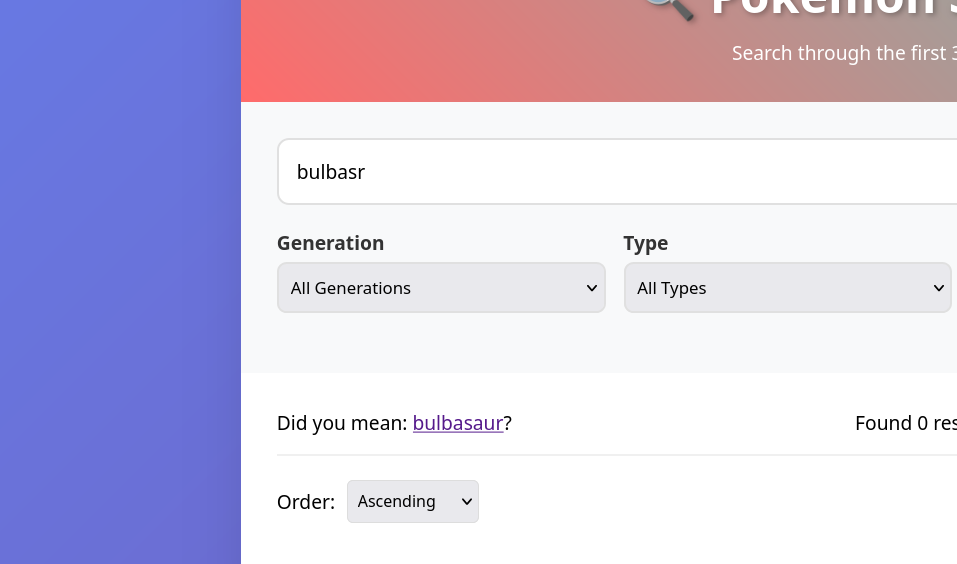
\includegraphics[width=0.7\textwidth]{figures/Screenshot_search_did_you_mean.png}
    \caption{Rechtschreibkorrektur-Feature bei der fehlerhaften Eingabe "`bulbasr"' mit "`Did you mean: bulbasaur?"'-Vorschlag basierend auf dem Solr SpellCheck-Component}
    \label{fig:spellcheck}
\end{figure}

Die Rechtschreibkorrektur-Funktionalität ist in Abbildung~\ref{fig:spellcheck} dargestellt. Bei der fehlerhaften Eingabe "`bulbasr"' erkennt das System automatisch den Tippfehler und bietet den korrekten Suchbegriff "`bulbasaur"' als klickbaren Link an. Diese Funktion basiert auf dem indexierten Vokabular und hilft Nutzern, trotz Eingabefehlern schnell zum gewünschten Ergebnis zu gelangen.

\subsection{Pokemon-Detailansicht und Modal-Interface}

Die Detailansicht für einzelne Pokemon wird über den \texttt{/api/pokemon/<id>} Endpunkt realisiert und bietet umfassende Informationen zu jedem Pokemon in einer Modal-Darstellung. Diese Implementierung ermöglicht es, detaillierte Informationen anzuzeigen, ohne die Hauptsuchseite zu verlassen und den Suchkontext zu verlieren.

\begin{figure}[htbp]
    \centering
    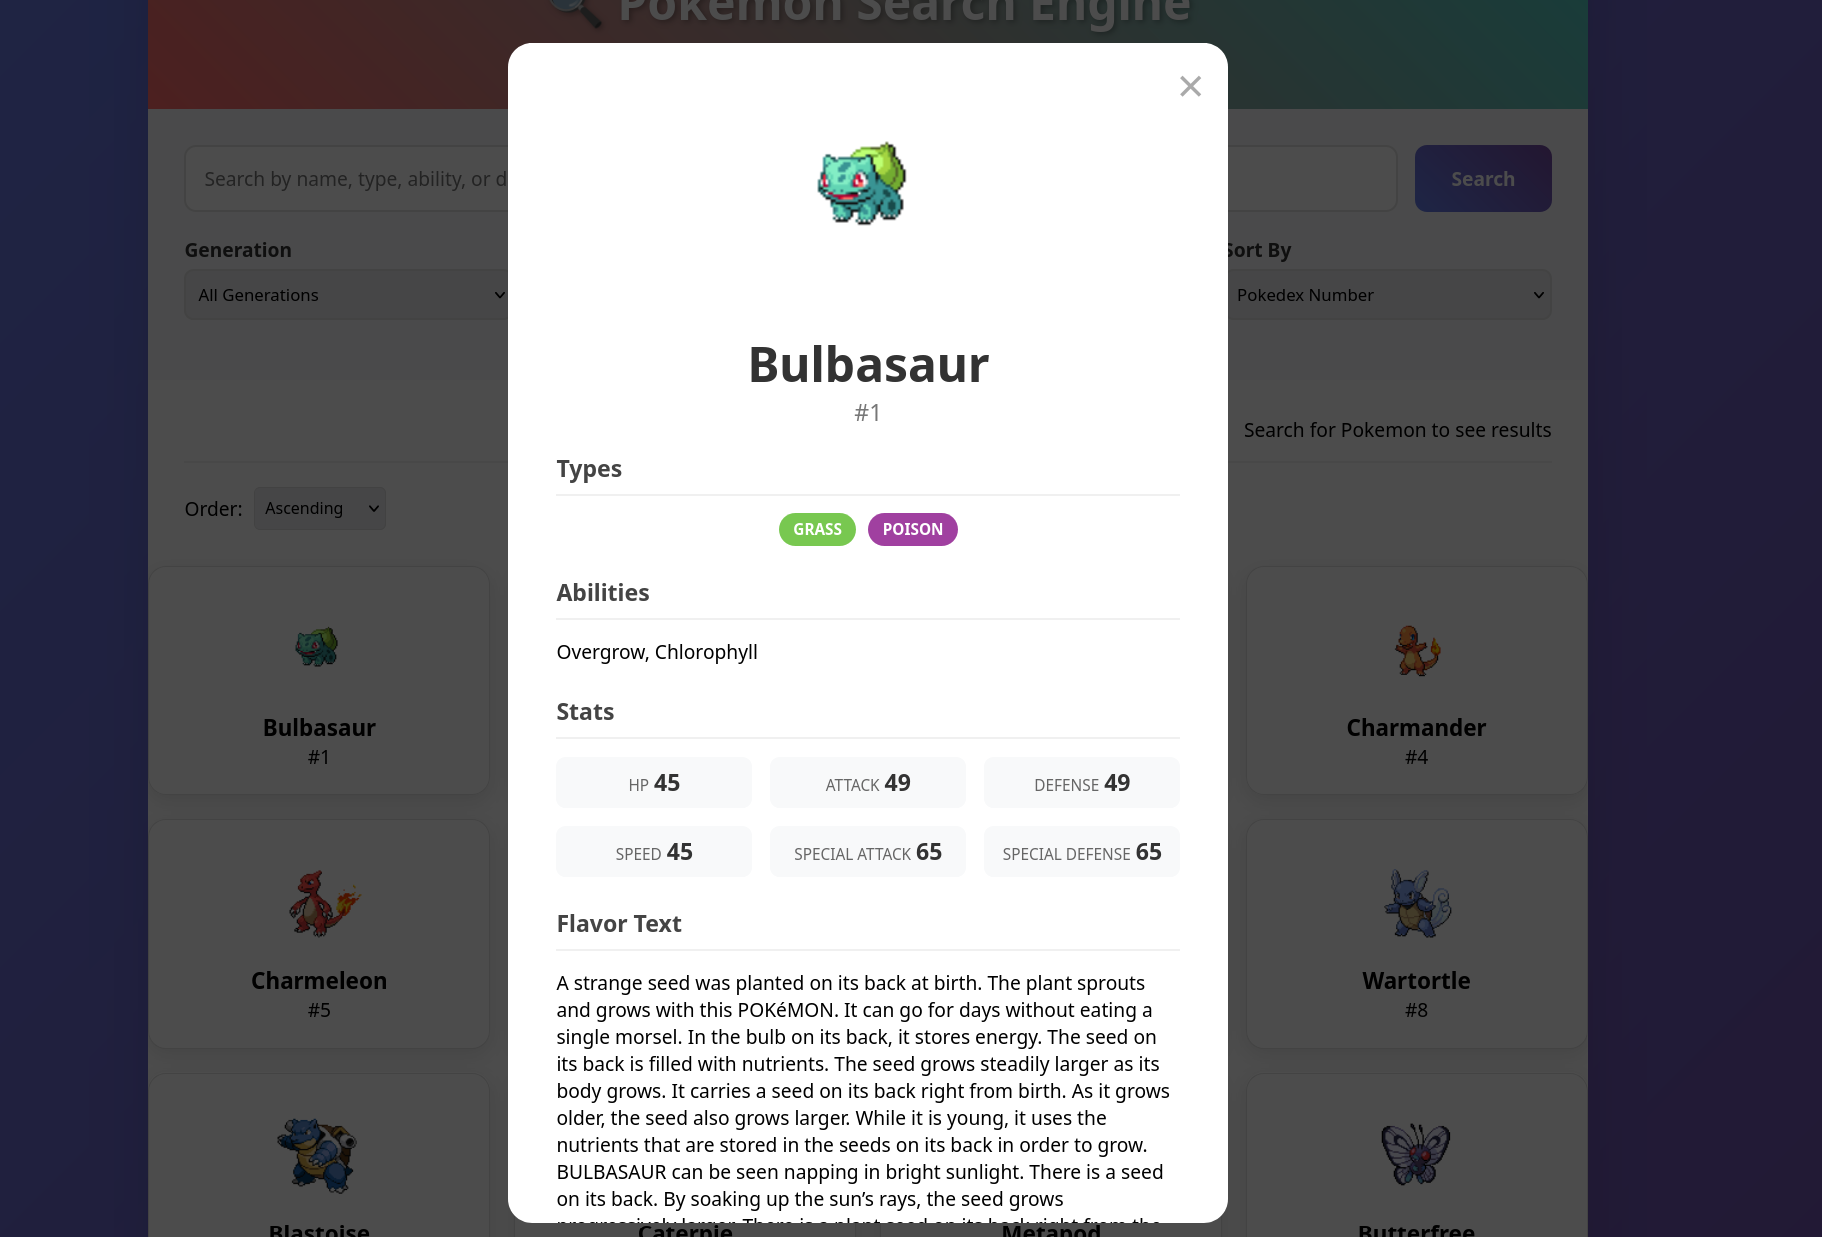
\includegraphics[width=0.85\textwidth]{figures/Screenshot_modal.png}
    \caption{Modal-Detailansicht für Bulbasaur mit vollständigen Pokemon-Informationen: Typen (Grass/Poison), Fähigkeiten (Overgrow, Chlorophyll), detaillierte Basis-Statistiken (HP, Attack, Defense, Special Attack, Special Defense, Speed) und Flavor-Text-Beschreibung}
    \label{fig:pokemon_modal}
\end{figure}

Abbildung~\ref{fig:pokemon_modal} zeigt die umfassende Modal-Detailansicht am Beispiel von Bulbasaur. Die Darstellung präsentiert strukturiert alle relevanten Pokemon-Daten: Typ-Badges für visuelle Erkennbarkeit, eine übersichtliche Auflistung der Fähigkeiten mit Unterscheidung zwischen normalen und versteckten Fähigkeiten, detaillierte Statistikwerte für alle sechs Basis-Stats und den vollständigen Flavor-Text aus den Pokemon-Spielen. Diese Modal-Implementierung bietet eine Balance zwischen Informationsdichte und Benutzerfreundlichkeit.

\subsection{Orchestrierung durch \texttt{main.py}}

Das Hauptskript fungiert als zentrale Koordinationsstelle für den gesamten Datenimport-Prozess. Nach der Initialisierung aller Komponenten -- \texttt{ApiClient}, \texttt{DataProcessor} und \texttt{SolrIndexer} -- erfolgt ein Solr-Verbindungstest und das Schema-Setup. Die iterative Verarbeitung aller Pokemon erfolgt generationsweise, wobei das Errorhandling den Gesamtprozess bei einzelnen Problemen nicht unterbricht.

Den Abschluss bilden Index-Optimierung und die Erstellung des Spellcheck-Dictionary, wodurch das System für optimale Suchperformance konfiguriert wird.


